\documentclass[12pt, a4paper]{report}
\usepackage{polski}
\usepackage[utf8]{inputenc}
\usepackage{amsfonts}
\usepackage{hyperref}
\hypersetup{
    colorlinks=true,
    linkcolor=black,
    urlcolor=blue,
    citecolor=black
}
\usepackage{float}
\usepackage{longtable}
\usepackage[compact]{titlesec}
\titleformat{\chapter}{}{}{0em}{\bf\LARGE}
\usepackage{lipsum}
\usepackage{graphicx}
\graphicspath{ {./wykresy/} }



\renewcommand{\contentsname}{Spis treści}
\renewcommand{\refname}{Bibliografia}

\title{Metody optymalizacji, lista 3}
\author{Radosław Wojtczak, numer indeksu: 254607}
\date{11.06.2023}
\begin{document}
\maketitle
\tableofcontents

\chapter{Wprowadzenie}
  W ramach listy numer 3 należało zaimplementować w języku programowania \textbf{julia} 2-aproksymacyjny
  algorytm oparty na programowaniu liniowym dla problemu szeregowania zadań na niezależnych maszynach
  z kryterium minimalizacji długości uszeregowania. W celu wykonania zadania skorzystano z pakietu JuMP.
  Algorytm został zaimplementowany w oparciu o książkę \cite{Alg}. Wszystkie szczegóły algorytmu 
  znajdują się w rodziale 17 (algorytm 17.5).

\chapter{Problematyka}
  Zaimplementowany algorytm jest sposobem na rozwiązanie problemu harmonogramowania zadań na niezależnych, równoległych
  maszynach (ang. Scheduling on unrelated parallel machines). Problem ten polega na przypisaniu 
  zbioru zadań do zbioru niezależnych, równoległych maszyn w taki sposób, aby minimalizować czas wykonania wszystkich zadań.
  W opisywanym problemie każde zadania ma określony czas wykoniania na każdej z rozpatrywanych maszyn.
  Przedstawiając powyższe w zwięzłej, matematycznej formie:
  \begin{itemize}
    \item J - zbiór zadań, $n = |J|$
    \item M - zbiór maszyn $m = |M|$
    \item p - macierz czasów realizacji zadania, zdefiniowana dla każdego zadania, które potencjalnie może zostać 
    wykonane dla każdej z maszyn 
    \begin{equation}
      (\forall j \in J) ((\forall m \in M) (p_{ij} \in \mathbb{Z}^{+} ))
    \end{equation}

  \end{itemize}
  Próbując utworzyć model programowania liniowego dla wskazanego problemu najlepiej zacząć 
  od konstrukcji modeulu programowania całkowitoliczbowego:
  \begin{itemize}
    \item $min \: t$, gdzie t sumarycznym czasem realizacji zadania na najdłużej pracujacej maszynie
    \item Każda z prac może być zrealizowana tylko na jednej maszynie
    \begin{equation}
      \sum_{i \in M} x_{ij} = 1 \: : \: j \in J
    \end{equation} 
    \item Każda z maszyn nie może pracować dłużej niż wskazuje na to minimalizowana zmienna \textit{t}
    \begin{equation}
      \sum_{j \in J} x_{ij} * p_{ij} \leq t \: : \: i \in M
    \end{equation}
    \item Zmienne decyzyjne okreslone są wartościami całkowitymi, gdzie wartość 1 oznacza, 
    iż i-ta maszyna realizuje j-tą pracę
    \begin{equation}
      x_{ij} \in \{0,1\} \: : \: i \in M, \: j \in J
    \end{equation}
  \end{itemize}
  Następnie chcielibyśmy dokonać relaksacji ostatniego ograniczenia, sprowadzającym tym samym problem do dobrze znanego 
  nam programowania liniowego, jednakże pojawia się problem, w którym optymalizator dokonuje niecałkowitego podziału prac między maszyny. 
  Aby wyeliminować powyżsża sytuację, autor pracy \cite{Alg} zaproponował następujący algorytm:
  \begin{enumerate}
    \item Przeprowadź wyszukiwanie binarne w przedziale [$\frac{\alpha}{m}$,$\alpha$].
    Znajdź najmniejszą wartość T na zbiorze liczb całkowitych dodatniych, dla której 
    LP(T) ma dopuszczalne rozwiązanie. Oznacz tę wartość jako $T^{*}$
    \item Znajdź rozwiązanie bazowe dopuszczalne x dla problemu $LP(T^{*})$
    \item Przypisz wszystkie zadania z wartościami całkowitymi do maszyn zgodnie 
    z rozwiązaniem x
    \item Skonstruuj graf i znajdź w nim doskonałe skojarzenie
    \item Przypisz zadania z wartościami ułamkowymi do maszyn zgodnie ze skojarzeniem
  \end{enumerate}
  Dzięki powyższemu algorytmowi, wcześniej przedstawiony model możemy sprowadzić do programowania 
  liniowego zastępując definicję zmiennych decyzyjnych w następujący sposób
  \begin{equation}
    x_{ij} \geq \{0,1\} \: : \: i \in M, \: j \in J
  \end{equation}
  Celem następnych sekcji jest eksperymentalne ocenienie jakości proponowanego algorytmu aproksymacyjnego.

\chapter{Otrzymane wyniki}
  Poniższa skrócona tabela przedstawia wyniki otrzymane w ramach przeprowadzonych testów na instancjach dostarczonych 
  przez bibliotekę "Instances for unrelated parallel machines problems and makespan criterion". Pełna tabela 
  przedstawiająca wyniki dla wszystkich instancji znajduje się na końcu pracy.
  \begin{table}[H]
    \centering
    \begin{tabular}{|c | c | c | c |} 
    \hline
    Instancja & OPT & Algorytm & 2*OPT\\
    \hline
    121 & 30.0 & 42 & 60.0 \\
    122 & 36.0 & 46 & 72.0 \\
    123 & 32.0 & 52 & 64.0 \\
    124 & 33.0 & 48 & 66.0 \\
    131 & 19.0 & 35 & 38.0 \\
    132 & 23.0 & 40 & 46.0 \\
    133 & 16.0 & 26 & 32.0 \\
    134 & 18.0 & 34 & 36.0 \\
    511 & 501.0 & 524 & 1002.0 \\
    512 & 484.0 & 501 & 968.0 \\
    \hline
    \end{tabular}
    \caption{Porownanie wybranych wyników optymalnych oraz wyprodukowanych przez algorytm dla wybranych instancji z rozpatrywanej biblioteki}
\end{table}
  Zgodnie z Twierdzeniem 17.8 \cite{Alg} wartości w kolumnie "Algorytm" nie powinny przekraczać dwukrotności algorytmu optymalnego. Na poniższym wykresie
  można zauważyć, iż faktycznie krzywa prezentująca wartości otrzymane przez algorytm znajduje się pomiędzy krzywą reprezentująca rozwiązanie optymalne oraz jego dwukrotność.
  \begin{figure}[H]
    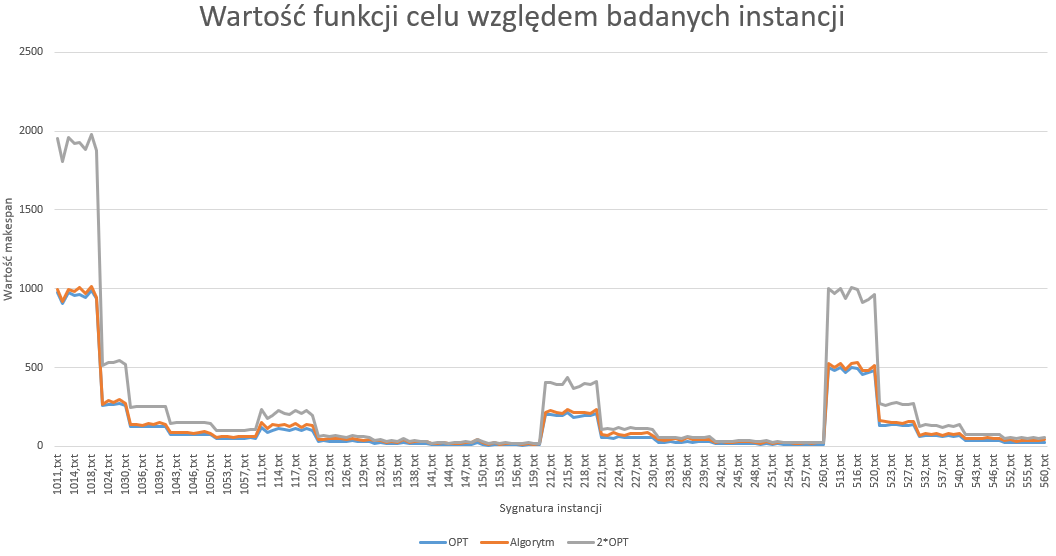
\includegraphics[scale=0.5]{1}
    \centering
    \caption{Wykres wartości funkcji celu względem wszystkich badanych instancji}
  \end{figure}
  \begin{figure}[H]
    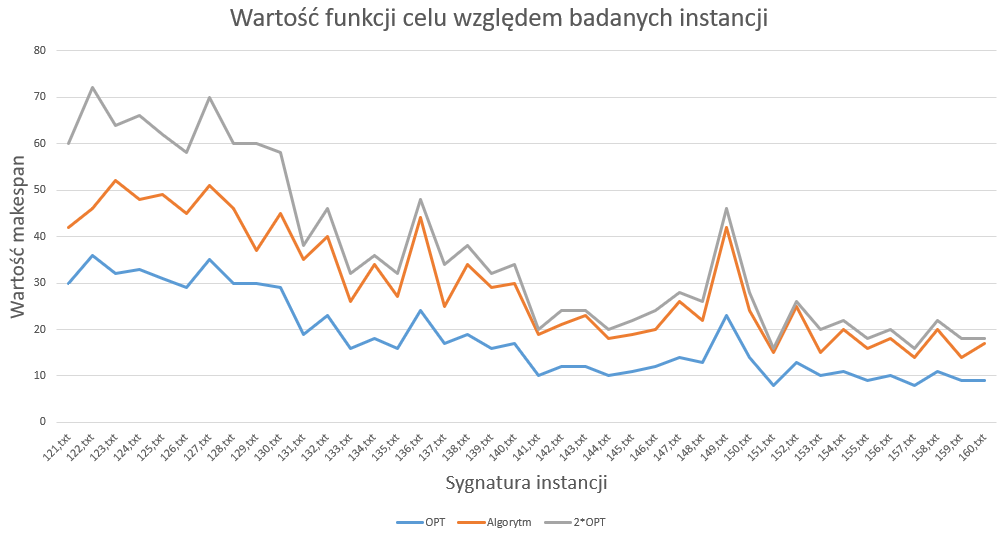
\includegraphics[scale=0.5]{2}
    \centering
    \caption{Wykres wartości funkcji celu względem wybranych instancji w celu polepszenia widoczności}
  \end{figure}
  Na podstawie powyższego wnioskujemy, iż prezentowany algorytm jest dobrym algorytmem aproksymacyjnym.
\chapter{Pełna tabela}
\begin{longtable}{| c | c | c | c |}
  \hline
  Instancja & OPT & Algorytm & 2*OPT\\
  \hline
  1011 & 977.0 & 997 & 1954.0 \\
  1012 & 905.0 & 919 & 1810.0 \\
  1013 & 978.0 & 995 & 1956.0 \\
  1014 & 960.0 & 985 & 1920.0 \\
  1015 & 964.0 & 1009 & 1928.0 \\
  1016 & 0 & 999 & 0 \\
  1017 & 942.0 & 971 & 1884.0 \\
  1018 & 990.0 & 1011 & 1980.0 \\
  1019 & 937.0 & 946 & 1874.0 \\
  1020 & 0 & 1011 & 0 \\
  1021 & 258.0 & 267 & 516.0 \\
  1022 & 0 & 278 & 0 \\
  1023 & 0 & 263 & 0 \\
  1024 & 266.0 & 288 & 532.0 \\
  1025 & 0 & 288 & 0 \\
  1026 & 267.0 & 279 & 534.0 \\
  1027 & 0 & 301 & 0 \\
  1028 & 272.0 & 296 & 544.0 \\
  1029 & 0 & 279 & 0 \\
  1030 & 260.0 & 275 & 520.0 \\
  1031 & 0 & 146 & 0 \\
  1032 & 0 & 154 & 0 \\
  1033 & 123.0 & 136 & 246.0 \\
  1034 & 126.0 & 138 & 252.0 \\
  1035 & 0 & 145 & 0 \\
  1036 & 125.0 & 135 & 250.0 \\
  1037 & 128.0 & 145 & 256.0 \\
  1038 & 126.0 & 136 & 252.0 \\
  1039 & 128.0 & 151 & 256.0 \\
  1040 & 127.0 & 138 & 254.0 \\
  1041 & 74.0 & 89 & 148.0 \\
  1042 & 0 & 85 & 0 \\
  1043 & 77.0 & 85 & 154.0 \\
  1044 & 75.0 & 89 & 150.0 \\
  1045 & 77.0 & 88 & 154.0 \\
  1046 & 75.0 & 84 & 150.0 \\
  1047 & 0 & 84 & 0 \\
  1048 & 75.0 & 85 & 150.0 \\
  1049 & 76.0 & 92 & 152.0 \\
  1050 & 74.0 & 83 & 148.0 \\
  1051 & 51.0 & 56 & 102.0 \\
  1052 & 49.0 & 60 & 98.0 \\
  1053 & 51.0 & 61 & 102.0 \\
  1054 & 51.0 & 58 & 102.0 \\
  1055 & 51.0 & 60 & 102.0 \\
  1056 & 0 & 60 & 0 \\
  1057 & 50.0 & 64 & 100.0 \\
  1058 & 0 & 59 & 0 \\
  1059 & 54.0 & 65 & 108.0 \\
  1060 & 52.0 & 61 & 104.0 \\
  111 & 117.0 & 152 & 234.0 \\
  112 & 87.0 & 111 & 174.0 \\
  113 & 98.0 & 136 & 196.0 \\
  114 & 115.0 & 131 & 230.0 \\
  115 & 104.0 & 136 & 208.0 \\
  116 & 101.0 & 125 & 202.0 \\
  117 & 114.0 & 147 & 228.0 \\
  118 & 103.0 & 122 & 206.0 \\
  119 & 114.0 & 139 & 228.0 \\
  120 & 98.0 & 131 & 196.0 \\
  121 & 30.0 & 42 & 60.0 \\
  122 & 36.0 & 46 & 72.0 \\
  123 & 32.0 & 52 & 64.0 \\
  124 & 33.0 & 48 & 66.0 \\
  125 & 31.0 & 49 & 62.0 \\
  126 & 29.0 & 45 & 58.0 \\
  127 & 35.0 & 51 & 70.0 \\
  128 & 30.0 & 46 & 60.0 \\
  129 & 30.0 & 37 & 60.0 \\
  130 & 29.0 & 45 & 58.0 \\
  131 & 19.0 & 35 & 38.0 \\
  132 & 23.0 & 40 & 46.0 \\
  133 & 16.0 & 26 & 32.0 \\
  134 & 18.0 & 34 & 36.0 \\
  135 & 16.0 & 27 & 32.0 \\
  136 & 24.0 & 44 & 48.0 \\
  137 & 17.0 & 25 & 34.0 \\
  138 & 19.0 & 34 & 38.0 \\
  139 & 16.0 & 29 & 32.0 \\
  140 & 17.0 & 30 & 34.0 \\
  141 & 10.0 & 19 & 20.0 \\
  142 & 12.0 & 21 & 24.0 \\
  143 & 12.0 & 23 & 24.0 \\
  144 & 10.0 & 18 & 20.0 \\
  145 & 11.0 & 19 & 22.0 \\
  146 & 12.0 & 20 & 24.0 \\
  147 & 14.0 & 26 & 28.0 \\
  148 & 13.0 & 22 & 26.0 \\
  149 & 23.0 & 42 & 46.0 \\
  150 & 14.0 & 24 & 28.0 \\
  151 & 8.0 & 15 & 16.0 \\
  152 & 13.0 & 25 & 26.0 \\
  153 & 10.0 & 15 & 20.0 \\
  154 & 11.0 & 20 & 22.0 \\
  155 & 9.0 & 16 & 18.0 \\
  156 & 10.0 & 18 & 20.0 \\
  157 & 8.0 & 14 & 16.0 \\
  158 & 11.0 & 20 & 22.0 \\
  159 & 9.0 & 14 & 18.0 \\
  160 & 9.0 & 17 & 18.0 \\
  211 & 204.0 & 213 & 408.0 \\
  212 & 204.0 & 230 & 408.0 \\
  213 & 197.0 & 216 & 394.0 \\
  214 & 195.0 & 211 & 390.0 \\
  215 & 218.0 & 236 & 436.0 \\
  216 & 183.0 & 212 & 366.0 \\
  217 & 189.0 & 217 & 378.0 \\
  218 & 198.0 & 214 & 396.0 \\
  219 & 197.0 & 211 & 394.0 \\
  220 & 206.0 & 232 & 412.0 \\
  221 & 55.0 & 76 & 110.0 \\
  222 & 58.0 & 68 & 116.0 \\
  223 & 53.0 & 85 & 106.0 \\
  224 & 60.0 & 76 & 120.0 \\
  225 & 55.0 & 69 & 110.0 \\
  226 & 59.0 & 82 & 118.0 \\
  227 & 58.0 & 79 & 116.0 \\
  228 & 56.0 & 79 & 112.0 \\
  229 & 58.0 & 89 & 116.0 \\
  230 & 54.0 & 69 & 108.0 \\
  231 & 27.0 & 45 & 54.0 \\
  232 & 27.0 & 40 & 54.0 \\
  233 & 28.0 & 42 & 56.0 \\
  234 & 27.0 & 48 & 54.0 \\
  235 & 24.0 & 36 & 48.0 \\
  236 & 31.0 & 57 & 62.0 \\
  237 & 27.0 & 43 & 54.0 \\
  238 & 28.0 & 44 & 56.0 \\
  239 & 29.0 & 45 & 58.0 \\
  240 & 30.0 & 46 & 60.0 \\
  241 & 17.0 & 26 & 34.0 \\
  242 & 17.0 & 31 & 34.0 \\
  243 & 16.0 & 25 & 32.0 \\
  244 & 17.0 & 25 & 34.0 \\
  245 & 19.0 & 34 & 38.0 \\
  246 & 18.0 & 33 & 36.0 \\
  247 & 18.0 & 28 & 36.0 \\
  248 & 17.0 & 27 & 34.0 \\
  249 & 14.0 & 21 & 28.0 \\
  250 & 18.0 & 28 & 36.0 \\
  251 & 13.0 & 21 & 26.0 \\
  252 & 16.0 & 27 & 32.0 \\
  253 & 12.0 & 23 & 24.0 \\
  254 & 12.0 & 22 & 24.0 \\
  255 & 13.0 & 21 & 26.0 \\
  256 & 12.0 & 20 & 24.0 \\
  257 & 13.0 & 22 & 26.0 \\
  258 & 12.0 & 21 & 24.0 \\
  259 & 13.0 & 25 & 26.0 \\
  260 & 12.0 & 23 & 24.0 \\
  511 & 501.0 & 524 & 1002.0 \\
  512 & 484.0 & 501 & 968.0 \\
  513 & 500.0 & 525 & 1000.0 \\
  514 & 469.0 & 488 & 938.0 \\
  515 & 503.0 & 528 & 1006.0 \\
  516 & 497.0 & 529 & 994.0 \\
  517 & 455.0 & 484 & 910.0 \\
  518 & 467.0 & 481 & 934.0 \\
  519 & 0 & 511 & 0 \\
  520 & 483.0 & 514 & 966.0 \\
  521 & 135.0 & 163 & 270.0 \\
  522 & 130.0 & 161 & 260.0 \\
  523 & 137.0 & 152 & 274.0 \\
  524 & 138.0 & 154 & 276.0 \\
  525 & 0 & 161 & 0 \\
  526 & 134.0 & 146 & 268.0 \\
  527 & 132.0 & 159 & 264.0 \\
  528 & 0 & 159 & 0 \\
  529 & 137.0 & 160 & 274.0 \\
  530 & 0 & 136 & 0 \\
  531 & 62.0 & 69 & 124.0 \\
  532 & 68.0 & 84 & 136.0 \\
  533 & 67.0 & 76 & 134.0 \\
  534 & 66.0 & 83 & 132.0 \\
  535 & 0 & 116 & 0 \\
  536 & 0 & 79 & 0 \\
  537 & 61.0 & 72 & 122.0 \\
  538 & 66.0 & 83 & 132.0 \\
  539 & 63.0 & 75 & 126.0 \\
  540 & 68.0 & 80 & 136.0 \\
  541 & 39.0 & 50 & 78.0 \\
  542 & 39.0 & 48 & 78.0 \\
  543 & 39.0 & 49 & 78.0 \\
  544 & 39.0 & 51 & 78.0 \\
  545 & 39.0 & 54 & 78.0 \\
  546 & 38.0 & 47 & 76.0 \\
  547 & 0 & 56 & 0 \\
  548 & 0 & 57 & 0 \\
  549 & 0 & 52 & 0 \\
  550 & 37.0 & 51 & 74.0 \\
  551 & 26.0 & 39 & 52.0 \\
  552 & 27.0 & 41 & 54.0 \\
  553 & 26.0 & 34 & 52.0 \\
  554 & 27.0 & 36 & 54.0 \\
  555 & 26.0 & 40 & 52.0 \\
  556 & 27.0 & 35 & 54.0 \\
  557 & 0 & 38 & 0 \\
  558 & 26.0 & 36 & 52.0 \\
  559 & 0 & 33 & 0 \\
  560 & 27.0 & 42 & 54.0 \\  
  \hline
  \caption{Porownanie wszystkich wyników optymalnych oraz wyprodukowanych przez algorytm dla wybranych instancji z rozpatrywanej biblioteki}
\end{longtable}
  Należy zauważyć, iż w każdym przypadku wartość $Algorytm \in [OPT,2*OPT]$, gdzie $OPT \geq 0$.





  \clearpage
  \phantomsection
  \addcontentsline{toc}{section}{Bibliografia}
  \bibliographystyle{plain}
  \bibliography{literatura}
\end{document}